


\section{女子寮生向けハラスメント相談窓口より}

%文責扱いで
\author{女子寮生向けハラスメント相談窓口} 

\subsection{はじめに}
こんにちは、女子寮生向けハラスメント相談窓口です。私たちは、熊野寮に住む女子寮生によって組織されていて、女子寮生が暮らしやすくなるように様々な活動を行っています。私たちのアプローチの対象は寮内の女性だけでなく、寮外の「熊野寮に入寮するかもしれない人たち」も包含しています。以下の文章は、私たちが、熊野寮生の出身校に送付することを目指して作成した冊子を加筆・修正したものです。

%タイトルみたいな形にしたい
\noindent{京都大学熊野寮女子寮生から高校生のあなたへ}

\vspace{3cm}

\begin{figure}[hbp]
\centering
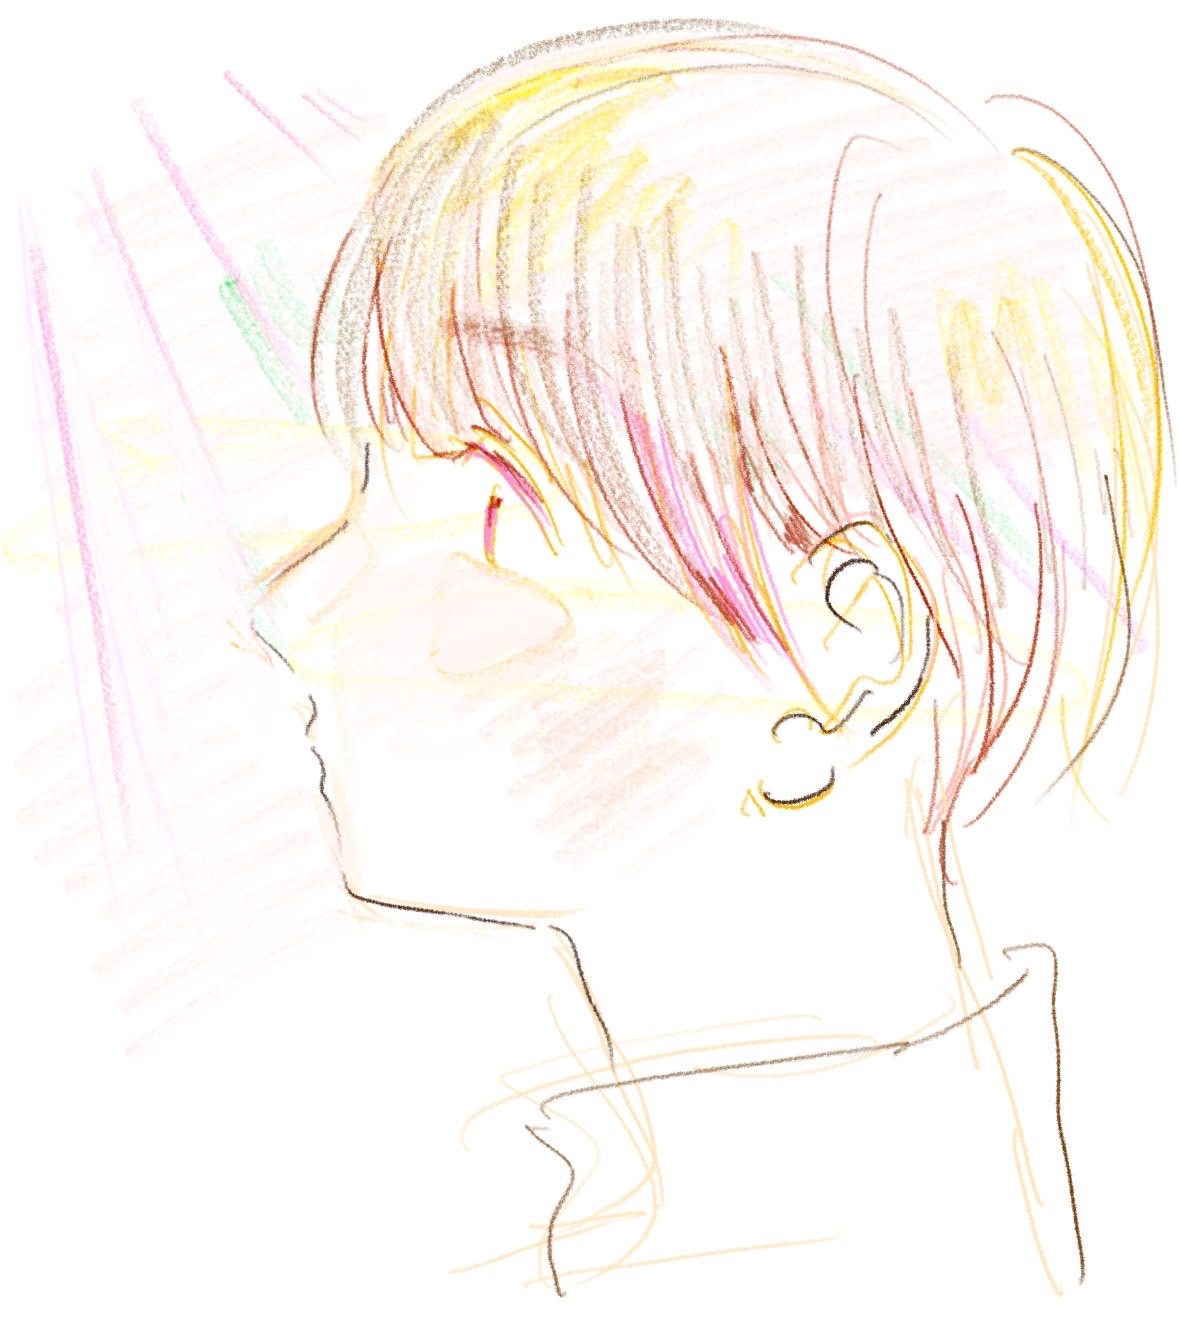
\includegraphics[width=8cm]{2025shinki/joshi_ryosei/kijigazo.jpg}
\end{figure}




\subsection{まえがきのようなもの}
\hfill {文責:翠}

\begin{flushleft}
あなたへ
\end{flushleft}
\vskip\baselineskip
まずは、この冊子を手に取ってくれたあなたに大きな感謝を。

この冊子は、京都大学の学生寮である熊野寮における女子寮生向けハラスメント相談窓口(以下、女子寮生窓口)という団体が主体となり、実際に寮に住む女子寮生の寄稿によって出来上がったものです。日本の高等教育では女子の比率は男子に比べて少なく、京都大学や私たちの住む熊野寮においても例外ではありません。熊野寮内において、女子寮生の数は全体の2割程度です。「女子 (ここで述べる女子(女性)とは、生物学的に女性の身体をもち、女子トイレや女子シャワー室を利用する人たちを指します)」という属性を持つ私たちはマイノリティであることを一つの理由として日々もやもやとした思いを感じることがあります。私たち女子寮生窓口のメンバーは、女子寮生が感じるそういった生きづらさ、住みづらさを解消するため、日頃は匿名での相談受付や女子寮生新歓の開催を行っています。そして、これから先の進路に迷ったり迷わなかったりしている高校生のあなたに、女性という属性を持つ人生の少し先輩として、今の生きづらさやこれから直面するであろう生きづらさに対処していくためのヒントが渡せたらいいなという思いから、この冊子を作り、届けることになりました。(もちろん、高校生でない方にも、京都大学の一学生が考えていることをふむふむと読んで楽しんでいただければと思っています。)
\vskip\baselineskip
現状、悲しいことですが、性差に基づく生きづらさが社会の中に存在しています。

女性を例に挙げると、女が勉強なんてとんでもないという価値観に縛られて大学や大学院に行きにくかったり、実家を離れて生活することに難色を示されたり、男女の夫婦関係において家事育児の負担を多く担っていてキャリアを犠牲にしたり、化粧やスカートの着用を強制されたり、満員電車や夜道に性被害の恐怖が伴ったり…。

でも、これは、女性だけの生きづらさではなく、男性と女性のどちらにも当てはまらない性の在り方をもっている人や男性においても、それぞれの人にとって形を変えて眼前に現れるものであると思います。女性の生きづらさの根源は、生物学的性に基づく、男らしさ女らしさの強制であり、多様な性的な在り方の否定です。あらゆる属性の人間1人1人がもつ大きな可能性を握りつぶす抑圧です。そういうのが、社会にはずーっと前から今まであり続けて、男性や女性やすべての人を息苦しくさせているのです。

私たち女子寮生窓口は形式上「女子」寮生向けとなって女性に焦点を当てているけれど、最終的には、男性もその他の性を持つ人も、むしろすべての人が性別に起因する生きづらさから解放されることを目指しているのじゃないかと思っています。少なくとも、私はそうあってほしいと思いながら活動をしています。20何年生きてきた私自身、自分が女であるということを否定できない事実として受け止めている一方で、今でも自分が性的にも社会的にも女であることを強く否定したい気持ちに襲われます。そういう男とか、女とか、関係ない社会になればいいのにね、という話です。

すこし大きな話をしてしまいましたが、これから先に掲載されている文章は熊野寮女子寮生や元寮生の日常的でささいな思いの表出です。こんな女性が京都大学にいて生活しているのだというロールモデルを提供できたらそれはとても嬉しいですし、あなた自身の人生において、やりたいことをやる後押しができたのなら、それはもっと嬉しいです。
\vskip\baselineskip
\begin{raggedleft}
かつてあなたと同じ境遇だったかもしれない私より
\end{raggedleft}
\newpage

\subsection{一人暮らしから熊野寮へ}
\begin{flushright}
総合人間学部 5 回生 H.O.
(2024 年春入寮)
\end{flushright}

\subsubsection{はじめに}
この文章は、この春、熊野寮に入った一人の女子寮生である私の生活について綴ったものです。「女性であること」についての言及はそこまで多くありませんが、この文章を読んで少しでも皆さんが「熊野寮に暮らす女性」をより鮮明にイメージでき、身近に感じるようになればいいなと思い、寄稿させていただきました。
\vskip\baselineskip
私が熊野寮に引っ越してきたのは、大学“5 回生”になる春休み、3 月末のことだった。もうすぐ4 月だというのに、冷たい風が吹き荒れて雪の舞う、寒さの厳しい夜。4 人部屋のルームメイトの 1人から手渡された合鍵を大事に握りしめて、これからの寮生活に胸を高鳴らせた。

\subsubsection{私が熊野寮に入るまで}
 私が京都大学に入学したのは 2020 年 4 月、新型コロナウイルス流行に伴う外出規制がちょうど始まった頃だった。大学の授業は全てオンラインだったので、1 回生の前期は福井の実家で過ごし、後期から京都に移り住んで、元田中駅近くの 1K のアパートで一人暮らしを始めた。それ以来、4 回生の終わりまで合計で約 3 年間(3 回生で半年留学をした期間は除く) 、私はそこで暮らした。白い床と白い壁の部屋に合うよう、家具は淡い木目調で揃えた。決して広くはないがかわいらしいその部屋を、私は気に入っていたはずだった。それなのにいつの間にか、私は部屋にいても落ち着かなく感じるようになってしまった。 「自分は一人暮らしよりも、誰かと一緒に住む方が幸せだろうな」 。ひとりで作った夕食を、iPad を相棒にして食べるとき、そんな考えが止められなくなったからだ。
\vskip\baselineskip
 留学の関係で 1 年留年して“5 回生”となった私は(大学に来てから知ったことだが、様々な理由で 4 年よりも長い時間をかけて学部を卒業する人というのはけっこういる)、大学生活最後の 1 年を過ごす場所として熊野寮を選んだ。1 回生の頃から「熊野寮祭」などのイベントに遊びに来て、寮が楽しい場所だと知っていたから、そこで多くの寮生と知り合いになったから…というだけなら、おそらく私は入寮には踏み切らなかった。かつての私にとって、熊野寮はあくまで「非日常」で「お祭り騒ぎ」の場所であり、自分がそのカオスの中で生活するイメージはまるでつかなかったからだ。転機となったのは、特別仲の良い友人が、昨年秋に寮に移り住んだこと。入寮後すぐ「友達はできたの?」と聞くと、満面の笑みで「大友達、大出来」と返ってきた。 「おおともだち……おおでき…。 」あまりに勢いの良い返事に呆気にとられながら、私は、今の自分が求めているのはこれなのではないかと思った。ひとりきりのご飯は虚しい。虚しさとは真逆のところに行ってみたい。人がいっぱいいて、それも皆個性的でバラバラで、いつもどこかで何かが起きていて、笑っちゃうくらい情報ぎゅうぎゅう詰めのところに。親友に寮の中を案内してもらい、それまで見たことのなかった炊事場や居室、シャワー室などの、寮生の居住エリアを一通り見せてもらった。壁の落書きやビラなど、たしかにゴチャゴチャしているけれど、これなら意外と普通に住めるかも、というのが感想だった。他のシェアハウスやドミトリーも検討していたが、 「熊野寮に住む」という選択肢が、一番わくわくした。当時の私の直感は間違っていなかったと、今振り返って思う。
\vskip\baselineskip

 2 月末の入寮面接を終え、無事、寮に住むことが決まったものの、引っ越しには苦戦した。3 年間の一人暮らしで溜め込んだ荷物を処理しきれないまま引っ越し当日を迎えた私は、初めて入る談話室\footnote[1]{同じ階(ブロック)の人が集まってくつろぐリビングのような部屋。ゲームをしたり映画を見たり漫画を読んだり課題をしたり、使い方は人によって様々である。}の引き戸を開けるなり真っ青な顔で「引っ越しを手伝ってくれませんか!?」と懇願する、迷惑な新入寮生と化した。 「あの…あと 1 時間で前のアパートの退去なんですけど、まだ…まだ中に荷物が残ってて…!」と、火事の建物に人が残されているかの如く切実に訴えた日のことが、昨日のように鮮明に思い出せる。幸い、その時談話室にいた同じ階の優しい住人たちのおかげで、私はなんとか熊野寮への引っ越しを完了したのだった。

\subsubsection{新歓と「居場所」の広がり}
 入寮してからの日々は、とんでもない速さで過ぎていった。春の間は怒涛のような新歓の連続で、新入寮生の私は、5 回生なのに行く先々で歓迎された。自分の 1 回生当時、コロナ禍で新歓がサークル活動ごとなくなってしまった分を余裕で取り戻すどころか、お釣りが来るくらいの歓迎されっぷりに驚いた。新歓といっても、アルコールを強要されたり嫌なノリを押し付けられたりすることはなく、ご飯やお菓子を囲んでおしゃべりする平和なものだ。各ブロックの新歓、部会や委員会の新歓、軽音にボードゲームなど趣味の集まりの新歓に加え、女性の寮生が集う「女子寮生新歓」というのもあった。ポトフやガパオライスなど、料理好きの寮生たちが腕を振るったとりどりの料理を一緒につつきながら、大学やバイトといった他愛もない話をして仲良くなった人たちとは、その後寮のシャワー室や食堂で顔を合わせたときにも言葉を交わす友人となった。こうしたコンパなどがきっかけで、寮の中に「ほっとする居場所」が作られていく感覚は幸せで、ありがたかった。

*

 あっという間に季節は過ぎて、12 月。入寮から 9 ヶ月が経とうとしている今、すっかり馴染んだ談話室のこたつで、私は筆を執っている。

\subsubsection{寮生として一度きりの「熊野寮祭」 、全てを詰め込んだ 10 日間}
 
先日まで、寮の最大のイベント「熊野寮祭」が行われていた。外から遊びに来るのではなく、寮の中の人間として参加する寮祭は、自分にとってこれが最初で最後。悔いのないよう楽しみ尽くそうと張り切った 10 日間は、それはもう盛りだくさんだった。ずっと出てみたかった名物企画「エクストリーム帰寮 \footnote[2]{夜中に車で知らない土地に降ろされた参加者が、地図・スマホ・現金を使わずに徒歩で熊野寮に帰ってくる企画。通称「エク帰」 。毎年 X(Twitter)等でも話題になる、熊野寮祭の名物企画。}」に友人とともに参加し、宇治から大津を経由して帰ってきたその足で、大量のスポンジケーキを並べて「ケーキコンパ\footnote[3]{スポンジケーキに好きなトッピングを載せて飾り付け、その独創性を競う企画。今年は「おいしい部門」 「美しい部門」 「ゲテモノ部門」の 3 部門で投票が行われた。}」を行った。ある夜は「方言マルチリンガル」になるという野望を掲げ、北は北海道弁・南は沖縄弁まで、全国津々浦々の方言話者と戯れた。またある夜は「福井県民コンパ」と称して、地元福井の名物を振る舞った。ある朝には早起きして、ホテルの朝食ビュッフェを自らの手で再現する企画のために、だし巻き卵を大量に巻いて…。寮祭について語ろうとすれば、紙面がいくらあっても足りない。ここまで挙げたのは、私自身が主体となって参加・運営した企画だけで、全体で 500 を超える寮祭企画のほんの一部にすぎないのだから。
\vskip\baselineskip

もう一つ、寮祭の中で忘れてはならない出来事が、音楽好きの寮生たちによる、3 日間にわたるライブだ。私は 3 日間で 3 つのバンドに出演し、うち 2 つでボーカル、1 つでドラムを担当した。私がドラムを務めるのは、なんと同じ部屋の人たちと一緒に組んだ“部屋バンド”。とある休日の朝、部屋で話していると「この部屋でバンドやりたくない?」という話になり、私は早速その日の午後に楽器屋に走ってドラムのスティックを買った。9 月初めのなんてことのない曇りの日が、部屋バンドの結成で急にきらきらと愛おしく輝きだしたのが懐かしい。1 年前の自分は想像しえただろうか?1 年後の自分が、同じ部屋の人とバンドを組み、ドラムを叩いてライブに出ているだなんて。不思議な世界線に生きているものだと、つくづく思う。
\vskip\baselineskip

 ライブや寮祭、コンパのような「ハレ」のまばゆいまでの楽しさと、毎日の寮食や談話室での会話のような「ケ」の中に散りばめられた喜び。それらを噛み締めて、1 日 1 日を大切に過ごしているつもりだけれど、きっと寮を出るまでの残りの日々も、忙しくてあっという間なのだろう。 「追いコン」で追い出される日も、きっとすぐだ。それまで、寮で出会った様々な人とのつながりを大切に、今、ここでしかできないことを追いかけるのだ。

\subsubsection{おわりに ―大学生活、どこに住もうか考えているあなたへ}
 一人暮らしには、一人暮らしの良さがある(入寮後、稀に、自分で自由に使えるきれいな個室が恋しくなる) 。人によって、共同生活が好きな人もいれば、一人暮らしの方が好きな人もいる。同じ共同生活でも、実家に家族と住むのか、シェアハウスに友達と住むのか、はたまた寮に住むのか、どんな寮なのか…選択肢はさまざまだ。この文章を読んで少しでも「熊野寮いいな、楽しそう!」とピンときた人は、きっと私のように、この寮を楽しむ素質のある人だ。そういう人にはもれなく、ぜひ一度寮に遊びに来てもらいたいと思う。

\vskip\baselineskip
 高校生の皆さんは、大学では一人暮らしを考えている人も多いだろう。まずは一人暮らしに挑戦してみる、という選択も一つだが、そのときに覚えておいてほしいのは、暮らし方は常に、ひとつではない、ということだ。今の暮らしとは別のところに、心躍る出会いが待っているかもしれない。もしも一人暮らしに飽きてしまったら、いつでも寮に来ればいい。熊野寮は、毎年春と秋の 2 回、入居者を募集している。この文章を読んでくれたみなさんの頭の隅に、 「熊野寮で暮らす」という選択肢が置かれるようになったなら、これ以上嬉しいことはない。

\newpage

\subsection{勇気をくれた仲間、大切な居場所}
\begin{flushright}
 文責:U.N. 
\end{flushright}

京大に入学してから、自身の「女性」という性別を意識する機会が増えた。意識するというより「させられる」という表現のほうが適切だろうか。大学そのものに加えて、私が自ら飛び込んだチャレンジングな環境は、往々にして女性が少なく男性が多い場所だった。その中でも、私にとって重要な居場所は2つある。第一に、進学と同時に入寮した熊野寮。第二に、進級を機に入部した、とある運動部。女性が言わば「マイノリティ」であるこれらの環境下で、気楽さや新鮮さを感じながら過ごす一方で、疎外感や自分・周囲に対する違和感を抱くことも少なからずある。
\vskip\baselineskip

今から紹介するのは、そのような私の経験談である。この文章が、性別や属性にまつわる各々の考察を深める何かしらのきっかけになれば幸いである。
\vskip\baselineskip

進級後の5月。新たに入部した運動部は寮と比較して、人数比の面でも、雰囲気の面でも、女性が「マイノリティ」であった。性別を問わず同じフィールドで競技できる運動部は珍しいが、だからこそ、身体的な構造の違いにより「女子部員」であることを意識させられることも多い。
\vskip\baselineskip

入部後の日々は充実しており、素晴らしい挑戦と思い出に満ちている。しかし、秋頃から部内のホモソーシャルな雰囲気が気になり始めて、不快な思いをする出来事もあった。先輩に相談した際のアドバイスも「上手くやり過ごす」「女子同士で愚痴を言い合って解決する」など、現状を変えるアクションが二の次にされていることに、心底驚いた。
\vskip\baselineskip

嫌なことを嫌なまま我慢したくない、それなら私が動こう、と部活の定例ミーティングで問題提起をしたところ、トップの組織から部の意識の改善を呼びかけてもらえた。
\vskip\baselineskip

「私が動こう」とは簡単に言ったものだが、自分が中心となって行動することは、考えていたより格段に難しく、エネルギーを消耗した。少なくとも寮の基準に照らし合わせれば、これがセクハラであり間違っていることは明確であったが、実際には、嫌という感覚を説明しても上手く共有できなかったり、周りの雰囲気に飲まれて自分の考えを主張しきれなかったりと、思い通りに行かないことが多かった。
\vskip\baselineskip

そのような歯がゆい思いをして初めて、「これはセクハラで」「間違っている」という自分の信念が、決して自分1人のものではなく、熊野寮という環境ありきで形成され、発動されてきたものだということが分かった。
\vskip\baselineskip

私の場合は部内にしがらみが少なく「ダメなら辞めてやる」ぐらいの潔さがあったので、たまたま行動を起こせた。しかし、もっと複雑な人間関係が絡んでいたり、金銭的理由が関与したり、その他何らかの事情で八方塞がりになってしまうことも、十分にありえたはずだ。実際、このように複雑な状況から、ハラスメント問題では安易に行動を起こすことが難しい・相談さえ憚られる場合が大半だ。行動を起こせるか否かは、個人の強さ/弱さによるものでは全く無く、その人を取り巻く環境や条件に大きく依存する。しかし本来、どんな場面であれ、泣き寝入りが強いられることは絶対にあってはならない。そのために必要なのは、問題を1人で抱え込まず、同じ志を持った仲間と力を合わせて現状を変えていくことだ。
\vskip\baselineskip

その仲間に出会えた場所が、私の場合は熊野寮だった。嫌なことは嫌、おかしいことはおかしいと抗議できる風土がここにはある。ハラスメントの問題に関しても、相談窓口や現場の対策の徹底で不快な出来事を防ぎ、新歓で繋がりを作り、万が一何か起こってしまっても被害者をケアし、再発防止に務めるという組織的な体制が出来上がっている。しかし、これは最初から「出来上がって」いたわけではないし、今でも決して完璧なものではない。先輩たちが議論と行動を重ねて作り上げてきたもの、私たちが不断の努力により、これからも作り続けるものである。
\vskip\baselineskip

私がこの文章を書いたのは、自らの経験談を「熊野寮は良いところだけど他の場所は居づらいよね」で終わらせないため、自分が享受しているある種の特権を自分以外の人へ、寮以外の場所へ広めてゆく足掛かりとするためだ。部活の話も、私の行動に対して応援や感謝をしてくれる人たちに支えられてこそのものであった。そうやって、互いに行動や応援をし合う仲間が増えれば必ず、現状をより良くすることができる。
\vskip\baselineskip

自分の大切な居場所でありながら、周りとの属性の違いが原因で嫌な思いをしてしまった時、できることが不当に制限されてしまった時、私たちはどうすれば良いだろうか。見ないふりをするか、黙って我慢するか、仕方ないと諦めるか、惜しみつつその居場所を離れるか。私は、Noと主張し、毅然と闘う道を選びたい。同時に、そのような道を、1人でも多くの人と共に歩みたい。
\vskip\baselineskip

とは言え、この文章を読んでくれた人にいきなり「力を合わせて現状を変えていく」ことを強いるつもりは全くない。自分の考えを深めたり、周囲で悩んでいる人の話を聞いてあげたりするだけでも十分だ。もちろん、違和感や反発を覚える人、行動の必要性を感じない人もいるだろう。「女性だから」「寮生だから」などと、あなたの属性だけで安易に賛同を強要することは絶対にしない。
\vskip\baselineskip

その上で、もし何か悩みを抱えた時、私たちはあなたの相談に乗ることができる。また、勇気を持って行動を起こしたいと思う時が来たら、必ずあなたを後押しする。あなたと直接の関わりを持てなかったとしても、この文章を力に代えてほしい。あるいは、これから一緒に関わりを作っていこう。私たち女子寮生有志は、いつでもあなたの仲間です。
\newpage
\subsection{寮生活を振り返って}
\begin{flushright}
文責:Y.M.
\end{flushright}


私は熊野寮に入寮して4年目になる。今まで約3年間の寮生活を振り返ってみると、本当に思い出が尽きない。引っ込み思案でなかなか人前に出ることができない私だったが、寮の同期がコンパに連れ出してくれたり、SCを2度やらせてもらったり、ブロックの談話室民があたたかく迎え入れてくれたりして、たくさんの人たちと交流し、仲良くさせてもらっている。
\vskip\baselineskip

寮で出会った多くの人たちの中でも、特に出会えてよかったと思う女性の先輩が2人いる。その2人はもう退寮してしまって、頻繁に会うことはできなくなってしまったが、それでも定期的に会っている。寮で一緒に生活しているときには、何度も悩みごとを聞いてもらった。話を聞いてもらうと抱えているすべての心配事が大丈夫に思えてきて、前向きになることができた。
 \vskip\baselineskip
 
私が談話室に居つくことができたのもその2人の影響が大きい。私が入寮して初めて談話室を見たときには、床で2,3人が眠っていて起きている2人は画面に食い入るようにゲームをしていた。そのとき談話室にいたのが全員男子だったのもあり、私にはこの場所は縁遠いなと思った。ブロック内の新歓で談話室に入った時には、緊張で咄嗟に「お邪魔します…」と私が言うと、まだ名前も知らなかった男の先輩に「そういうのいいから、」と言われた。その言葉がとても冷たく感じ、なにか責められているような気がして、その後の新歓ではずっと縮こまってしまっていた。
\vskip\baselineskip

大好きな先輩2人と仲良くなってからは、談話室に行くと話せる人がいる、という安心感からよく談話室に通った。ゲームをしたり雑談をしたり、美味しいご飯を食べたりと幸せな時間だった。少し怖く感じていた談話室の人々も、話してみると楽しくて、談話室が大好きな場所になった。
 \vskip\baselineskip
 
今年も新入寮生がたくさん入ってくる。あの2人が私にしてくれたように、入ってくる後輩に居心地が良いと思ってもらえるように頑張りたい。いつの間にか自分より下の代が増えてきて先輩として頼られることへの不安もあるし、自分の進路の実現を考えると周りを気に掛ける余裕があるのかも不安なところであるが、自分ができるだけのことを精いっぱいやろうと思う。
\newpage

\subsection{同期座談会}
\subsubsection{メンバー紹介(仮名)}
ナス:総合人間学部4回生。歌が上手い。

トマト:医学部人間健康科学科4回生。踊るのが好き。

キャベツ:工学部4回生。リコーダーが吹ける。

\subsubsection{大学の中での女子}
トマト:みんなそれぞれ学部の毛色が違うから面白そう。

ナス:総人\footnote[1]{総合人間学部の略称。}に関しては大体半々、または男女比6:4くらい。とりわけ女子が少ないという雰囲気はない。総人はクラスの繋がりが薄いから、他の学部の話の方が参考になるかも。

キャベツ:工学部は女子はだいたい1割くらい。クラスのつながりは強くはないが、実験とかあって、そこだとだいたい班に女子1人。きついけど、きつくない状態を知らないから。。クラスで女子が少数だからこその結束はあるけど、クラスの内で仲良くなれないと大変かも。女子3人しかいないクラスもある。研究室に配属されたらまた感覚は変わるかも。寂しさを感じやすい気はする。

ナス:うちのゼミが、先生も先輩も男性ばかり。後輩には女子もいるが。改めて振り返ると女子1人だなと思う。

トマト:人健\footnote[2]{人間健康科学科の略称。}は、自分は特に看護だから、逆に男子1割しかいない。人健全体だともうちょっと男子がいて男4女6とかだと思うけど、京大の中ではあり得ない比率。男子は肩身狭そう。

キャベツ:逆に男子が数少なくて結束力強かったりするのかな。

トマト:結束力は強い。でもグループになるときは男子1人で大変そう。特別な役割を担わされがち。

ナス:もう少し研究室の話をすると、学部とかゼミとかは良いけど、人文学系のエリアにおいて専門性が高くなるにつれて、男性ばかりになっていく気がする。アカデミアの世界で段々女子が振り落とされていくなと思う。院進するなり博士にいくなり、ただでさえハードルがある上に女子が少ないとさらに行きにくさがある気がする。学問の道をバリバリ進むことにいちいち引っかかる感じがする。

キャベツ:京大で女子が3割しかいないこと等にも表れてるけど、勉強するのってどちらかというと男子で、男子の方がアカデミアに進むみたいな、そういう風潮はあるよなと思う。女子は就職後の結婚出産とか考えると、アカデミアに進むのがハードル高いのもありそう。ポスドク\footnote[3]{ポストドクターの略。大学院博士課程を修了したあとに、教授のような正規の立場ではなく、非正規の任期付きで研究員をしている人のこと。}とか、どこに転勤になるのかわからないとかもあるし、難しさがある。

ナス:ロールモデルの不足もあると思う。セクハラとかまでいかなくても、ちょっとナンセンス\footnote[4]{ 不適切な発言や態度を指していう言葉。}じゃないかみたいなのが積み重なる。そういう中で、上り詰めていくときにちょっとなと思うことが増えていくと思うと、アカデミアの道に進んでいく気が失せてしまう。

トマト:看護の話。看護は女性ばかりの学問領域だから、ロールモデルは豊富。それでもあり得ない経歴の人が多い。育休中に博士号取った人とか。30代前半で子どもを産み、せっかく休みだし博士号取ろうとなったらしい。大学にいる人はそんな人ばかり。女性としてのライフイベントを着実に達成しながら、結婚して子育てしながら研究もするみたいな。そういうのを聞くと、すごいと憧れるのと同時に、それは協力的なパートナーや親がいるとか、あなたがラッキーだったからではと思ってしまうところもある。自分にラッキーな状況があるとは限らない。だから諦めがちになるというか、葛藤がすごくある。

ナス:親との折衝もあった。学部卒が当たり前と言われていた。ほんとは親は大学も家から出す予定はなくて、そこを押し切ったから、就職は家に戻ることになった。そこが逆風だった。今振り返るとそういう環境にいたから、大学院に進む選択肢も浮かびにくかった。

キャベツ:そういうのが当たり前だった、ってことか。

ナス:研究で接する人は優しくしてもらっていて、社会人になってからでも戻ってきなよと言ってくれる人もいる。やや心残りがある。

キャベツ:大学の女友達とはつながりが薄めだからな。寮のコミュニティがあるからどうにかなっている。クラスだとコミュニティは狭くなりがちだから、みんなサークルとかに入るんだと思う。

トマト:まとめ。なんとなく女子が少なかったりする状況はあるけど、日々通っている中では実感はない。授業行くだけだから、ぱっと割り当てられたグループとかでは授業をするという目的があるからそんなに。アカデミアという観点では、ライフイベントを考えると選択しにくさがあったり、ロールモデルがいなかったり現実的じゃなかったりして考えにくい状況がある。私は親も自由にやらせてくれているし、アカデミアに残ることが出来る。環境に結構左右されるよね。

\subsubsection{1人暮らしについて}
トマト:ナスが親元を離れる予定はなかったと言っていたが。

ナス:熊野寮に入った経緯を言うと、安かったし、人がいるので安心というのがあった。アパートも検討したが、コロナもあり、知らないところに1人でいたら寂しいけど、寮ならみんないて安心というのはある。どちらかというと、お金が理由。おばあちゃんに心配されて、男女同じフロアか、セキュリティは、など。うまく説明した。私は一人娘なのもあって、過保護なんだよね。大事な一人娘なんだからねと言われることもあるけど、そこはもやっとする。心配されるのは娘だからなのか、子どもだからなのかわからない。でも実際、女性ゆえに夜道で襲われるリスクとかはあるし。

キャベツ:それは襲ってくる方が悪いんだけどね。

ナス:家出てなかったらどうなってたんだろうって考えることある。何も知らないまま大人になってたかも。女の子だから夜道気をつけよう、で終わっていたかも。諸々の気づきが無かったと思うと、ありがたいと同時に恐ろしいなと思う。かわいい子には旅をさせよ、だね。

トマト:家を出て良かったと思う。寮という場所は大変勉強になる場所。親元を離れた暮らしということ以上に、自分の生き方とか立場とかよく考えさせられるから、そういう意味で成長の機会をもらったと思う。私は家族が好きだけど、同時にしがらみだなとも感じる。最近帰省すると、私は家族だとどうしてもお姉ちゃんでいちゃうなと思う。家族内での「私」があって、帰る度につらいなと思う。そういう家族の中での「私」みたいなのを除いて、私としての私として生きていける瞬間が寮にはあるから、それが良いなと思う。

キャベツ:それはそうだなと思う。私は、実家を出たくて京大にきた。実家はかなり厳しかったし、実家から大学に通っていたら、まじめに勉強だけしていたと思うし、自分がやりたいと思ったことをあまりできなかったと思う。自分で考えて生きるっていうのが、寮に来て色んな人と出会ってできるようになった。家族の中の役割を担ってしまうというのはある。実家ではお父さんの機嫌を取らなきゃというのもあったし。寮に入って考えさせられるという話もあったけど、自分が自由な場所に身を置いているから考えられる。おかしいことにはおかしいと思っていいんだとか、思えるようになった。ありがたい環境。

ナス:さすがに寮入って良かった。学生寮は学生のうちしか入れなくて、1人暮らしはいつでもできる。

トマト:寮はやめられます。

キャベツ:一度入ってみたらいいのはそう。

ナス:私たちの仲間にも寮を卒業した人たちもいるけど、割と元気そうにやってるし。

キャベツ:もし寮を出ても、寮での関係性は続けることができる。

ナス:たまに集まって飲んだりもするしね。

\subsubsection{家族の中でのわたしたち}
キャベツ:今まで育てられてきた中で、女だからどうこうと言われたとかそういうのはどうだった?とかお母さんどうだった?というのは話したい。うちでは、両親の間に明確に権力差があって、お父さんが偉かった。小さい頃はそれが特異だと思っていたけど、他の寮生と話していて、そういう権力差のある家庭は割とあるのかなって。

ナス:権力差とまでは感じないが、母が専業主婦で父がサラリーマン。金銭面は父頼り。家事、育児は母がやっている。そういう意味ではお互い支え合っている。役割は明確に分かれている。母が専業主婦だったから女性が働くロールモデルが中高くらいまではあまり見えづらかった。ご飯作るのも大変なのに会社に行ったらもっと大変だと思っていた。

キャベツ:結婚と同時に仕事をやめた?

ナス:ちょっとはやっていたけど、ほぼ寿退社みたいな感じ。

トマト:私の家では、共働きで、妹が介護が必要だから、母親が介護もしてかつ働いて、家事もやってという感じ。女性が働くイメージは全然あった。ただ、父は仕事以外やらない感じだった。休日も、昔は遊んでくれたりしたけど、今は自分の趣味ばかりで、全然家庭のことをするという感じでない。母は強いと思う一方で、男は使えないという感覚があった。父とか旦那さんに期待しない方が良いのではと思っていた。だから、全部自分で出来るようになりたいと思っている。それに伴うプレッシャーもあるけれど。

ナス:人となりに家庭環境が影響を与えているのはある。トマトの話を聞いて顕著に思った。

キャベツ:うちも母が専業主婦だから、小さい頃は働く女性のイメージはなかった。うちの母は仕事辞めなきゃよかったって言っていて、そこから、強くなりたいとは思ったかな。経済的に父親が握っている、お父さんは稼いでいるから偉いみたいな感じがあって、勉強もできた。だから、私は将来稼いでやると思っていた。いつかお父さんをぎゃふんと言わせてやろうと勉強も頑張った。
ただ最近思うようになったのは、勉強頑張ったからといってぎゃふんと言わせられるわけじゃないんだろうなということ。結局は父親と娘だから。功績をあげたから関係が変わるとかではなく、自分の気の持ちようだなと。寮に来て、家から離れて、お父さんに思っていたこと(従わなきゃ、という気持ちなど)がなくなるから、一旦そこから引いて見れるようになった。家に帰ったら従っちゃうけど、従わなくてもいいんだなとか絶対的に偉い存在じゃないんだなって、思えるようになった。

ナス:うちとけっこう似てるところある。父親の考えが極端。18年間はその言葉を浴びるのが普通だと思っていた。家の狭い中だとその言葉から逃れられない。計画性がない、考えて行動しろと言われ続けてきた。もうちょっとアドリブでも良いし、やってみないと分からないこともあるじゃんと思う。家に戻ったら家のモードに戻ってしまうのもすごいわかる。4年経って、寮での自分を家に持ち帰れる余裕が出来てきた。権力差がないと言ったけど、そういう意味では父が強い面もあったのかな。それを見直せる場所と人と出会えて良かったなと思う。

トマト:家の中の私たちと外の私たちはあるよね。

キャベツ:家を出て気づけることってほんとにあるな。特に寮という環境に出てきたから気づけたこと多い。

ナス:また別の話だが、家に帰ると、熊野寮では弾劾されるような会話がいっぱいある。

キャベツ:社会にはナンセンスなこといっぱいあるよね。それをナンセンスだと認識して、言えるようになったのは、強くなれたのかなと思う。

トマト:ナンセンスだと認識してもうまく言えない。むかつくっていうので終わってしまう。

ナス:少なくとも座談会の場とかで共有できる。共有できるのが大事な上で、それで終わって良いのか、本来はそうじゃないよねというのはある。熊野寮という環境は大きい。熊野寮で身につけた感覚を、寮の空間内なら適応できるが、例えば部活で男子が多い中でちょっとなと思う場面があっても、言えなかったりする。自分の中の信念さえもねじ曲がっていく感じがある。寮というこの空間がすごいちゃんとしている。熊野寮でもまだまだ至らないところは無数にある上で、それでもなお、この男女比と人々の集まりようで大分ましなのは、すごく特殊だなと感じた。

トマト:寮の外でナンセンスだよとか言うと冷やかされそうとか、矮小化されて終わることが多い。女の子相手でもそう。何をあなたはでかい声で話しているのと言う感じの空気になったりする。理解を得られない。受け止めてすらもらえないこともある。勇気がいる。

ナス:からかわれるみたいなやり取りは厄介。「これハラスメントになっちゃうから良くないよね」とか、茶化して矮小化する感じ。「今の時代は厳しいから~」みたいな、意識してますみたいな感じ、めっちゃむかつく。

キャベツ:駄目だからダメなのではなく、それで嫌な思いをする人がいる、その場にいることすら難しくなる人がいるという切実性があるから、ハラスメントは駄目ってなっているはずなのに。駄目だからダメっていうのは、ただ、その人が自分を守っているだけで、傷つけちゃダメという意識がないのが怖いなと思う。

\subsubsection{寮内の議論について}
トマト:前提として、寮ではいろんなことが話し合いによって決められるべきとされている。何か問題が起こったら議論で解決してくださいと言う前提がある。その上で、議論が成立しないことも多い。さっきも言ったけど、問題意識を持ってこれを扱いたいですと言ったときに矮小化されたり、明後日の方向の意見がついて疲弊している人をたくさん見てきた。

キャベツ:寮生と話していて、問題の矮小化は無自覚に起きるのだなということは思う。一概にそうと言いたいわけではないけど、例えば、男子寮生と女子寮生におんなじ話をした時に、捉えられ方が違うというようなこととかある。その人の持っている属性で経験してきたことが全然違うから、違う属性に対してはだいぶ慎重にならないと矮小化になっちゃうんだなって感じる。

ナス:女子寮生の暮らしづらさについて一度会議で話したことがある。議場に持ち込んだときに、こちらの切実性が伝わりにくい。議論という場で、論理的にどうかということが重視されがちであるという印象をうける。プロセスの話になりがちだったり、個人の感情や思いを伝えにくかったり。プロセスの話をされ過ぎて、問題意識の共有が出来ず悲しい、とかいうのが共有できない。悲しいと思っている人がいます、と伝えるのがせいぜいで、自分の気持ちは主張しづらい。寮って結構、寮のために何ができるかという観点で議論を進めるけれど、暮らしやすさについて語るときは、個人の感情に基づくものだから、議論として扱うのは難しい。

キャベツ:感情を議論に持ち込むハードルが高いのは感じる。でも、寮生1人1人が暮らしづらいと思うのは、個人の話には留まらない。1人がそう思っていれば、他にも同様の意見を持っている人がいる可能性は高い。女子寮生新歓で、話してみたら共感を得られたとかもあるし、議場に上げにくさはあるとは言え、上げていかなきゃいけないんだろうな。感情の根拠をできるなら論理的に説明していく必要がある。個人の感情だからって無視されていたら、何も変わっていかない。

トマト:私はずっと言っていることがあって、私は感情でしか語れないから感情で議論したい。感情って、エネルギー。そういうエネルギーの放出の仕方が大きいから、今困っているとか、今モヤモヤしているとか、納得できないとか、そういう思いがある。でもそれをそのまま話すと伝わらないから、具体的に話さないといけなくなる。

キャベツ:もやもやとか、困ってますっていうのって、なんでですかとか、じゃあどうしていきたいんですかとか聞かれると言語化難しい。感情を議論に持ち込んじゃいけないというのはナンセンスだと思う。感情を話し始めたら議論を進めにくくなるというのはわかるけど。

ナス:持ち込んじゃいけない感情と、無視できない感情がある。トマトの言っている感情は話し合いにおいて正当な感情だと思う。一律に感情を持ち込んじゃいけないというのは違う。
全体的に、住みづらい、もやもやするみたいなのを議場に上げにくいのがある。この座談会も非公式的に行われている。発信はされるだろうが。こういう場があるだけでも十分と思う一方で、これがオルタナティブになっちゃっているのが悔しい。議論、議場、論理とかの話し合いで熊野寮が構成されていて、それが当たり前とされている。議論というフォーマットから漏れ出るものが取り残されがち。だから女子寮生相談窓口\footnote[5]{女子寮生向けハラスメント相談窓口のこと。}とか座談会とかが大事。会議の場とかでこういう話は出来ない。でもこれがうちうちに留まっていて外に出せなくなってしまう。

トマト:熊野寮の難しいところだね。

キャベツ:寮祭パンフ\footnote[6]{毎年11月末から12月の頭の10日間で開催される寮祭に際して発行されるパンフレット。企画のタイムスケジュールや注意事項が記載されている。}や入寮パンフ\footnote[7]{このパンフレットのこと。毎年2月ごろ、春の入寮者にむけて作成される熊野寮入寮情報や寮生の記事が掲載される。熊野寮ホームページで閲覧可能}のはじめにも「ハラスメント加害者にならないために」とかある。ああいうのってある程度論理的に、みんなが嫌だと思わないためにどうするかっていうのを書いているのかなって。ああいうものにつなげていくために、まずはもやもやを言える場所を増やすのが大事かなと思う。人と話して、整理されて、仲間がいる安心感から強気に外に出せるようになっていったりもする。そういうのもあって、女子寮生の集いとかもやってみたけど、女子に限らずいろんな寮生のもやもやを聞いてみたい。

ナス:もやもやコンパ\footnote[8]{コンパとは、熊野寮において、寮生が主に飲食を伴って交流する場。いわゆる合コンとは無関係。}とかしたら良いのでは。

トマト:ある程度前提を共有していたり、価値観が一緒だったりしないと、モヤモヤを話してもパンチ\footnote[9]{ここでの「パンチされる」とは、議論の場で大なり小なりの(建設的でない)批判や攻撃を食らうことを指す。主張した内容が不当に軽く扱われ、取り沙汰してもらえないというニュアンスを含む。「一蹴される」に近い。}されてしまう。でも、もやもやコンパのアイデアは面白いかも。そのぐらいざっくばらんに思いを語れる場が必要。私たちは女子の立場だが、属性によらずモヤモヤはある。例えば、生きるの辛い、大学行きたくない等…

キャベツ:前提を共有した上で言える場が必要。そもそもパンチされないことが理想だけど。なかなか難しい。

トマト:こうなんだよと言われたときにそうなんだねというワンクッションがあるだけで全然違うのに。とりあえずパンチ返されている人とかいるし、そういうのを見ていると自分も言いづらくなる。

ナス:パンチする以外の仕方を知らないとかもあるだろうな。優しい対応の仕方を教えると言っても、教える方が損するから難しいけど。

キャベツ:優しくできない人にも、背景はいろいろあるから、頭には入れておかないとなと思う。

\subsubsection{高校生の皆さんへ。}
トマト:長くなってしまったが、締めに向けて。まずは読んでくれてありがとうございます。皆色んな境遇あると思う、読んでいる人が男子か女子か分からないが、少なくとも熊野寮という環境はすごく自分を開発する、啓発する、発見する、新しい自分が見つかる場所。だから、興味持ったら熊野寮にきてくれるとよい。そうじゃなくても進む道で新たな出会いがあることを願っています。みなさんの進む先に幸があらんことを。 

ナス:いろいろ言ったけど、難しい部分もありつつ、熊野寮はいろんな人と出会えて、価値観も刷新される素晴らしい場。女子寮生という立場から言えば、もやもやを共有できる場所がある。不十分かもしれないけど、絶対ある。そういう場が確保されているということは安心材料になると思う。皆さんの入寮をお待ちしてます。困ったことがあったら一緒に考えていきましょう。ぜひ一度おいでください。

キャベツ:みんなが言うように、熊野寮は良い場所だし、すごい場所。よかったら、読んでいる人もぜひ熊野寮に来てくれたら嬉しい。熊野寮の良さは、人がいて、イベントがあって、いろんなことできて楽しいというのもあるけど、強く思うのは常識にとらわれないところ。当たり前とされているからそうすべきとかじゃなくて、何が良いかをみんなで考えて、変えるべきところはみんなの力で変えていけるというのが、熊野寮が社会の中の他の多くの場所よりもすごいと思うところ。もちろん寮の中でまだまだ改善点はあるが、もし読んでいる人が熊野寮に来たらぜひ一緒に寮を良い方向に変えていこうって言いたい。熊野寮に入らなくても、寮は寮生だけの場所ではなく、遊びに来ることもできるので。寮内にも寮外と連携しようという動きや、一緒に何かやろうという動きもある。遊びに来てくれたら。

(以上)

\newpage

\subsection{ババアになって茶ァしばこう}
\begin{flushright}
  文責:愚鈍羊、迷ちゃん
\end{flushright}

株式会社なる組織で仕事というものをしている身としてのこと、東京という土地に住所を置く身としてのこと、そういうことについて考えたほうが良いだろうし、言葉にしたほうがいいのかもしれない。「(女として)」と添えながら。筆者は熊野寮で6年暮らして、そのあと東京で働いて2年目を迎えている人間です。

書くことは山ほどあるのだと思う。やっぱり女の上司は少ないとか、私企業の枠組みで語られるハラスメント研修はクソだとか、あとは、醜悪な広告のこととか、あと東京都の子宮頸がんワクチンのキャッチアップ接種を受け損ねてどうしようと思っていることとか(自費は10万とかする)、そういうこと。 けれどもあまり筆が乗らないので、いつかどこかで書こうかなと思っていたことを思い出してみる。スカートを履かなくなった幼稚園児の頃のこと、(制服以外の)スカートを自分の選択で履けるようになった頃のこと、私より賢かったかもしれないが彼女の父によって望む進路を選べなかった母のこと。けれどそれも今言葉にされることを待っている事柄たちではないような気がしている。機を逸してしまったというか、またそのうち来るんだろう。

そこまでぼやぼや思いを巡らせて、文って宛先がないと書けないなァ~となる。読んでくれるかもしれない人、つまり寮で出会った人たち、今も寮にいるかもしれない人たち、これから寮で暮らすかもしれない人たちと、私はどういう話をしたいんだろう。

いやーーーーーー、まっじでわかんねー。

どうにか奮闘して寮を後にした人にも、今もなんとか寮で息をしている人にも、これから寮で暮らす選択をする/せざるを得ない人にも、何を言ったらいいのか、何か言えることなんてあるのか。漫画のめんどくさい主人公みたいなことなんぞ言いたかないのだが、でもほんとに私は寮にいる間、色んなことについて分かることはおろか、想像することもできなかったり、聞くこともできていなかったりした。

ただ、それでも、それなのに、私はこれから(も)寮で出会った女たちに助けられながら生きていくんだと思う。どうにか生活していくこと、行動すること、怒ることを私は彼女たちから知ったし、彼女たちの言うことが分からなくて学んだこと、考えたこと、想像したこと、それで得た言葉や知恵や感情のおかげで私はかつてより少し自由で少し強い。そんで、これからもっと自由で強いババアになりてぇ。
\vskip\baselineskip

ほんとうは、私より若いすべての女たちと、かつて私よりも若かったすべての女たちに捧げる言葉を持ちたかった。まだまだこれからですね。少し、長生きします。





